\subsection{Linear Algebra Primer}
\textbf{Motivation:} Getting rid of convolution and trying to use multiplication. 

\subsubsection{Eigenvalues and eigenvectors}
\begin{definition}
    Let \( V \) be a vector space over \( \mathbb{C} \) (or \( \mathbb{R} \)), let \( T: V \rightarrow V \) be a linear transformation. 
    \vspace{1em}

    A scalar \( \lambda \in \mathbb{C} \) (or \( \mathbb{R} \)) is called an eigenvalue of \( T \) if \( T(v) = \lambda v \) for some non-zero vector \( v \in V \) (v is then called an eigenvector associated with \( \lambda \)).
    \begin{itemize}
        \item \textbf{Note:} Helps understand \( T \): \( T \) acts on \( v \) by scaling them.
    \end{itemize}
\end{definition}

\begin{example}
    Suppose $V = \mathbb{R}^2$ with $T: \mathbb{R}^2 \to \mathbb{R}^2$ defined so that:
    \[
    \begin{pmatrix} x \\ y \end{pmatrix} \xrightarrow{T} \begin{pmatrix} 2 & -1 \\ 0 & 1 \end{pmatrix} \begin{pmatrix} x \\ y \end{pmatrix} = \begin{pmatrix} 2x - y \\ y \end{pmatrix}
    \]
    
    For the vector $\begin{pmatrix} 1 \\ 1 \end{pmatrix}$:
    \[
    T \begin{pmatrix} 1 \\ 1 \end{pmatrix} = \begin{pmatrix} 1 \\ 1 \end{pmatrix} = 1 \cdot \begin{pmatrix} 1 \\ 1 \end{pmatrix}
    \]
    Thus, $\lambda_1 = 1$ is an eigenvalue of $T$, and every non-zero multiple of $\begin{pmatrix} 1 \\ 1 \end{pmatrix}$ is a corresponding eigenvector.
    \vspace{1em}

    For the vector $\begin{pmatrix} 1 \\ 0 \end{pmatrix}$:
    \[
    T \begin{pmatrix} 1 \\ 0 \end{pmatrix} = \begin{pmatrix} 2 \\ 0 \end{pmatrix} = 2 \cdot  \begin{pmatrix} 1 \\ 0 \end{pmatrix}
    \]
    Thus, $\lambda_2 = 2$ is an eigenvalue of $T$, and every non-zero multiple of $\begin{pmatrix} 1 \\ 0 \end{pmatrix}$ is a corresponding eigenvector.
    \vspace{1em}

    Let $v_1 = \begin{pmatrix} 1 \\ 1 \end{pmatrix}, v_2 = \begin{pmatrix} 1 \\ 0 \end{pmatrix}$. If $v = \alpha_1 v_1 + \alpha_2 v_2$, then:
    \[
    T(v) = T(\alpha_1 v_1 + \alpha_2 v_2) = \alpha_1 T(v_1) + \alpha_2 T(v_2)
    \]
    \[
    = \alpha_1 \lambda_1 v_1 + \alpha_2 \lambda_2 v_2
    \]
\end{example}

\begin{intuition}
    This shows that a change of basis diagonalizes $T$, which helps simplify computations, especially for larger matrices.
\end{intuition}

\subsection{Key Fact}
\begin{definition}
    Complex exponential signals are eigenfunctions of LTI systems.

    \customFigure[0.5]{00_Images/EF.png}{Eigenfunction.}
\end{definition}

\subsubsection{Laplace Transform with Eigenfunctions in CT}
\begin{definition}
    \begin{equation}
        y(t) = e^{st} H(s)
    \end{equation}
    \begin{itemize}
        \item \( H(s) \) is the two-sided Laplace transform of \( h(t) \), defined as: $H(s) = \int_{-\infty}^{\infty} h(\tau) e^{-s\tau} d\tau$
    \end{itemize}
\end{definition}
\begin{derivation}
    In a CT system, consider the input \( e^{st} \) to a LTI system \( h(t) \), which produces the output \( y(t) \). Let $s \in \mathbb{C}$

    \begin{center}
    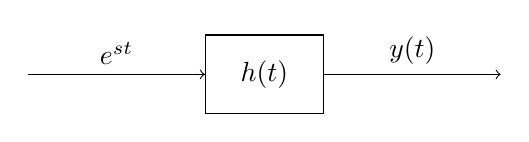
\begin{tikzpicture}
        \node at (0,0) [draw, rectangle, minimum width=1.5cm, minimum height=1cm] (H) {$h(t)$};
        \draw[->] (-3,0) -- (H) node[midway, above] {$e^{st}$};
        \draw[->] (H) -- (3,0) node[midway, above] {$y(t)$};
    \end{tikzpicture}
    \end{center}

    \[
    y(t) = e^{st} \ast h(t) = e^{st} \ast h(t)
    \]

    \begin{itemize}
        \item By commutativity of convolution, \( h(t) \ast e^{st} = e^{st} \ast h(t) \).
    \end{itemize}
    \vspace{1em}

    The convolution integral is:

    \begin{align*}
    y(t) &= \int_{-\infty}^{\infty} h(\tau) e^{s(t-\tau)} d\tau \\
    &= e^{st} \int_{-\infty}^{\infty} h(\tau) e^{-s\tau} d\tau \\
    &= e^{st} H(s)
    \end{align*}

    \begin{itemize}
        \item \( H(s) \) is the two-sided Laplace transform of \( h(t) \), defined as: $H(s) = \int_{-\infty}^{\infty} h(\tau) e^{-s\tau} d\tau$
    \end{itemize}
    \vspace{1em}

    Thus, the system simplifies to:

    \begin{center}
    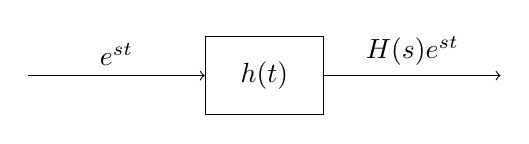
\begin{tikzpicture}
        \node at (0,0) [draw, rectangle, minimum width=1.5cm, minimum height=1cm] (H) {$h(t)$};
        \draw[->] (-3,0) -- (H) node[midway, above] {$e^{st}$};
        \draw[->] (H) -- (3,0) node[midway, above] {$H(s) e^{st}$};
    \end{tikzpicture}
    \end{center}

    \[
    \therefore e^{st} \text{ is an eigenfunction with eigenvalue } H(s).
    \]
\end{derivation}

\subsubsection{General Input}
\begin{derivation}
    Now, let \( x(t) \) be a sum of exponentials:

    \[
    x(t) = \alpha_1 e^{s_1 t} + \dots + \alpha_m e^{s_m t}
    \]

    Passing \( x(t) \) through the system \( h(t) \):

    \begin{center}
    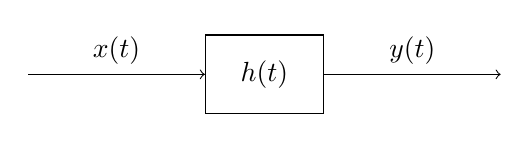
\begin{tikzpicture}
        \node at (0,0) [draw, rectangle, minimum width=1.5cm, minimum height=1cm] (H) {$h(t)$};
        \draw[->] (-3,0) -- (H) node[midway, above] {$x(t)$};
        \draw[->] (H) -- (3,0) node[midway, above] {$y(t)$};
    \end{tikzpicture}
    \end{center}

    \[
    y(t) = \alpha_1 H(s_1)e^{s_1 t} + \dots + \alpha_m H(s_m)e^{s_m t}
    \]
    \begin{itemize}
        \item We determine \( y(t) \) without convolution, making use of the eigenfunction and linearity, where each \( e^{st} \) is an eigenfunction of the system.
        \item \textbf{Note:} Since cosine and sine is a sum of complex exponential signals, it should be of the above form with different phase or magnitude, but no new frequencies.
        \begin{itemize}
            \item \textbf{Test for Linearity:} If you put a cosine in, you should get a cosine out. If not, it's non-linear. 
        \end{itemize}
    \end{itemize}
\end{derivation}

\subsection{Eigenfunction in DT}
\subsubsection{Z-Transform System with Eigenfunctions}
\begin{definition}
    \begin{align*}
        y[n] = z^n H(z)
    \end{align*}
    
    \begin{itemize}
        \item \( H(z) \) is the Z-transform of \( h[n] \), defined as: $H(z) = \sum_{k=-\infty}^{\infty} h[k] z^{-k}$.
    \end{itemize}
\end{definition}
\begin{derivation}
    In DT, consider the input \( z^n \) where \( z = e^{s} \) is passed through a LTI system with impulse response \( h[n] \), which gives output \( y[n] \).

    \begin{center}
    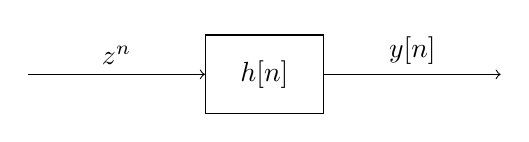
\begin{tikzpicture}
        \node at (0,0) [draw, rectangle, minimum width=1.5cm, minimum height=1cm] (H) {$h[n]$};
        \draw[->] (-3,0) -- (H) node[midway, above] {$z^n$};
        \draw[->] (H) -- (3,0) node[midway, above] {$y[n]$};
    \end{tikzpicture}
    \end{center}

    \[
    y[n] = z^n \ast h[n] = h[n] \ast z^n = \sum_{k=-\infty}^{\infty} h[k] z^{n-k}
    \]

    \begin{align*}
    y[n] &= z^n \sum_{k=-\infty}^{\infty} h[k] z^{-k} \\
    &= z^n H(z)
    \end{align*}

    \begin{itemize}
        \item \( H(z) \) is the Z-transform of \( h[n] \), defined as: $H(z) = \sum_{k=-\infty}^{\infty} h[k] z^{-k}$.
    \end{itemize}

    Thus, the system simplifies to:

    \begin{center}
    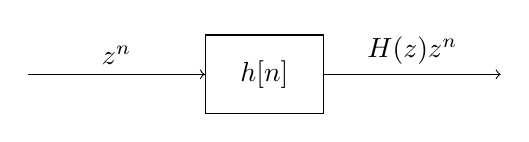
\begin{tikzpicture}
        \node at (0,0) [draw, rectangle, minimum width=1.5cm, minimum height=1cm] (H) {$h[n]$};
        \draw[->] (-3,0) -- (H) node[midway, above] {$z^n$};
        \draw[->] (H) -- (3,0) node[midway, above] {$H(z) z^n$};
    \end{tikzpicture}
    \end{center}

    \[
    \therefore z^n \text{ is an eigenfunction with eigenvalue } H(z).
    \]
\end{derivation}

\subsubsection{General Input}
\begin{derivation}
    Now, let \( x[n] \) be a sum of exponentials:

    \[
    x[n] = \alpha_1 z_1^n + \dots + \alpha_m z_m^n
    \]

    Passing \( x[n] \) through the system \( h[n] \):

    \begin{center}
    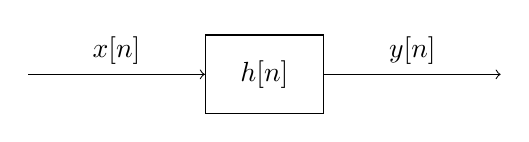
\begin{tikzpicture}
        \node at (0,0) [draw, rectangle, minimum width=1.5cm, minimum height=1cm] (H) {$h[n]$};
        \draw[->] (-3,0) -- (H) node[midway, above] {$x[n]$};
        \draw[->] (H) -- (3,0) node[midway, above] {$y[n]$};
    \end{tikzpicture}
    \end{center}

    \[
    y[n] = \alpha_1 H(z_1) z_1^n + \dots + \alpha_m H(z_m) z_m^n
    \]

    \begin{itemize}
        \item We determine \( y[n] \) without convolution, where each exponential function \( z^n \) acts as an eigenfunction of the system.
    \end{itemize}
\end{derivation}

\begin{warning}
    Now we want to levereage this property by decomposing all signals into a complex exponential form.
\end{warning}

\subsection{T-Periodic Signals of Complex Exponential Signals in CT}
\begin{definition}
    A complex exponential signal \( e^{(j2\pi f + \alpha)t} \) is \( T \)-periodic if and only if:

    \begin{enumerate}
        \item \( \alpha = 0 \)
        \item \( e^{j 2\pi f t} = e^{j 2\pi f (t + T)} \quad \forall t \)
        
        \begin{align*}
        e^{j 2\pi f t} &= e^{j 2\pi f t} e^{j 2\pi f T} \\
        \Longleftrightarrow 1 &= e^{j 2\pi f T} \\
        \Longleftrightarrow f T &= \text{integer}
        \end{align*}
        
        Therefore, \( f \in \left\{ \frac{0}{T}, \frac{1}{T}, \frac{2}{T}, \dots \right\} \) or equivalently \( f T = k \in \mathbb{Z} \).
        \begin{itemize}
            \item \textbf{Note:} $fT$ needs to be an integer since $2\pi f T$ represents the angle on the complex plane, we need it to be 1, which is only 1 for $2\pi k$ (i.e. when $fT=k$)
        \end{itemize}
    \end{enumerate}
\end{definition}

\subsubsection{Complex Exponential Fourier Series}
\begin{definition}
    Every linear combination of \( T \)-periodic signals is again \( T \)-periodic. All signals of the following form are \( T \)-periodic:
        \[
        x(t) = \sum_{k \in \mathbb{Z}} c_k e^{j 2\pi \left(\frac{k}{T}\right) t}
        \]
    \begin{itemize}
        \item \( f = \frac{k}{T} \).
        \item \( \left\{ e^{j 2\pi \left(\frac{k}{T}\right) T} : k \in \mathbb{Z} \right\} \): Basis set.
        \item \( c_k \in \mathbb{C}\): Coordinates (i.e. Fourier series coefficients)
        \item These are like a linear combination of a set of basis vectors.      
        \item Most signals can be represented in this form, but not all signals (we will only be focused on complex exp Fourier series though.)
    \end{itemize}
\end{definition}

\subsection{Inner product}
\begin{definition}
    Let \( x, y \in \mathbb{C}^{\mathbb{R}} \) be \( T \)-periodic signals, then
    
    \[
    \langle x, y \rangle = \frac{1}{T} \int_T x(t) y^*(t) dt
    \]
    \begin{itemize}
        \item $\int_T$: Integral taken over any length \( T \)-interval (e.g. $[0,T)$, $[-T/2,T/2)$)
        \item \( y^*(t) \) denotes the complex conjugate of \( y(t) \).
    \end{itemize}
\end{definition}

\subsubsection{Properties of Inner Products}
\begin{definition}
    \begin{enumerate}
        \item $\langle x, y \rangle \in \mathbb{C}$; if $\langle x, y \rangle = 0$ then we say $x, y$ are orthogonal.
        \item $\langle x, x \rangle = \frac{1}{T} \int_T |x(t)|^2 \, dt$, \quad $\langle x, x \rangle \in \mathbb{R}^{\geq 0}$; \quad $\langle x, x \rangle = 0$ iff $x \overset{a.e.}{=} \text{zero}$.
        \item $\langle x, y \rangle = \langle y, x \rangle^*$ \quad or \quad $(x, y)^* = \langle y, x \rangle$ \quad (i.e. Hermitian symmetry).
        \item For any scalars $\alpha, \beta \in \mathbb{C}$, \quad $\langle \alpha x, \beta y \rangle = \alpha \beta^* \langle x, y \rangle$.
        \begin{itemize}
            \item \textbf{Proof:}
            \begin{align*}
                \langle \alpha x, \beta y \rangle &= \alpha \langle x, \beta y \rangle \\
                &= \alpha \langle \beta y, x \rangle^* \\
                &= \alpha \beta^* \langle y, x \rangle^* \\
                &= \alpha \beta^* \langle x, y \rangle
            \end{align*}
        \end{itemize}
        \item Let $w, x, y, z$ be $T$-periodic signals, $\langle w + x, y + z \rangle = \langle w, y \rangle + \langle w, z \rangle + \langle x, y \rangle + \langle x, z \rangle$.
    \end{enumerate}    
\end{definition}

\subsubsection{Inner product of general signals}
\begin{definition}
    More generally, if $\{x_i : i \in I\}$ and $\{y_j : j \in J\}$ (i.e., finite/countable sets of $T$-periodic signals), then

    \[
    \left\langle \sum_{i \in I} a_i x_i, \sum_{j \in J} b_j y_j \right\rangle = \sum_{i \in I} \sum_{j \in J} a_i b_j \langle x_i, y_j \rangle
    \]
    \begin{itemize}
        \item i.e. inner product of sums is the sums of inner products.
    \end{itemize}
\end{definition}

\subsubsection{Inner product of complex exponential signals}
\textbf{Motivation:} Want to find the inner product of our basis set for Fourier analysis.
\begin{definition}
    For any $k, \lambda \in \mathbb{Z}$, the inner product of $e^{j 2\pi \frac{k}{T} t}$ and $e^{j 2\pi \frac{\lambda}{T} t}$ is

    \begin{align*}
        \left\langle e^{j 2\pi \frac{k}{T} t}, e^{j 2\pi \frac{\lambda}{T} t} \right\rangle =
        \begin{cases}
            1, & \text{if } k = \lambda \\
            0, & \text{if } k \neq \lambda
        \end{cases}
    \end{align*}
    \begin{itemize}
        \item \textbf{Note:} This result shows that the orthogonality condition is satisfied for complex exponentials with distinct frequencies.
        \item \textbf{Note:} This shows that our basis set builds an orthonormal system.
    \end{itemize}
\end{definition}

\begin{derivation}
    For any $k, \lambda \in \mathbb{Z}$, the inner product of $e^{j 2\pi \frac{k}{T} t}$ and $e^{j 2\pi \frac{\lambda}{T} t}$ can be calculated as follows:

    \begin{align*}
        \left\langle e^{j 2\pi \frac{k}{T} t}, e^{j 2\pi \frac{\lambda}{T} t} \right\rangle &= \frac{1}{T} \int_T e^{j 2\pi \frac{k}{T} t} \cdot \left(e^{j 2\pi \frac{\lambda}{T} t}\right)^* \, dt \\
        &= \frac{1}{T} \int_T e^{j 2\pi \frac{k}{T} t} \cdot e^{-j 2\pi \frac{\lambda}{T} t} \, dt \\
        &= \frac{1}{T} \int_T e^{j 2\pi \frac{(k-\lambda)}{T} t} \, dt \\
        &= \frac{1}{T} \int_T \cos\left(2\pi \frac{(k-\lambda)}{T} t\right) \, dt + j \frac{1}{T} \int_T \sin\left(2\pi \frac{(k-\lambda)}{T} t\right) \, dt \\
        &= 
        \begin{cases}
            1, & \text{if } k = \lambda \\
            0, & \text{if } k \neq \lambda
        \end{cases}
    \end{align*}

    \bigskip

    Now, let's plot the functions $\cos\left(2\pi \frac{(k-\lambda)t}{T}\right)$ and $\sin\left(2\pi \frac{(k-\lambda)t}{T}\right)$.

    \begin{center}
    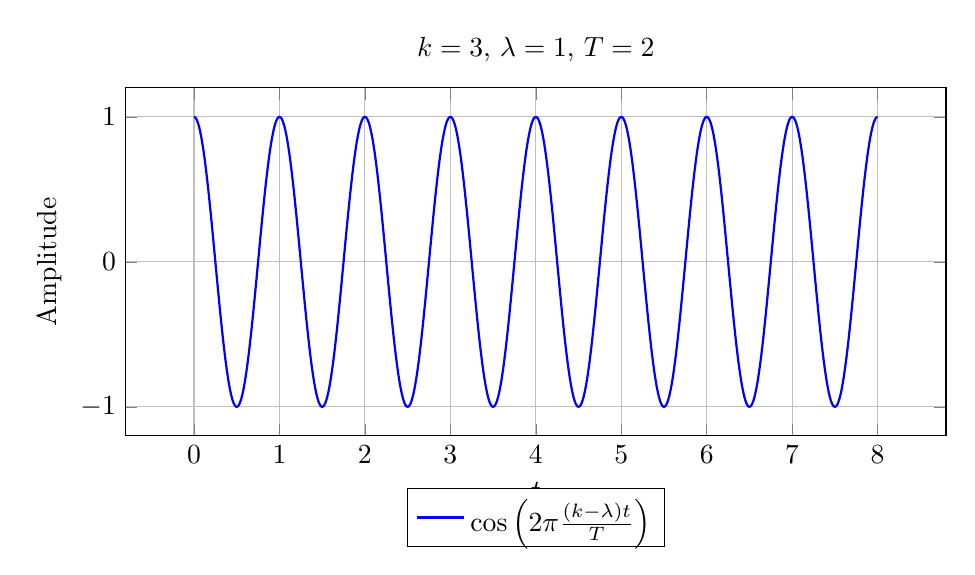
\begin{tikzpicture}
        \begin{axis}[
            width=12cm,
            height=6cm,
            grid=both,
            title={$k=3$, $\lambda=1$, $T=2$},
            xlabel={$t$},
            ylabel={Amplitude},
            legend style={at={(0.5,-0.15)}, anchor=north,legend columns=-1},
        ]
            \addplot[blue, thick, domain=0:8, samples=1000] {cos(deg(2*pi*(3-1)*x/2))};
            \addlegendentry{$\cos\left(2\pi \frac{(k-\lambda)t}{T}\right)$}
        \end{axis}
    \end{tikzpicture}
    \end{center}

    \begin{center}
        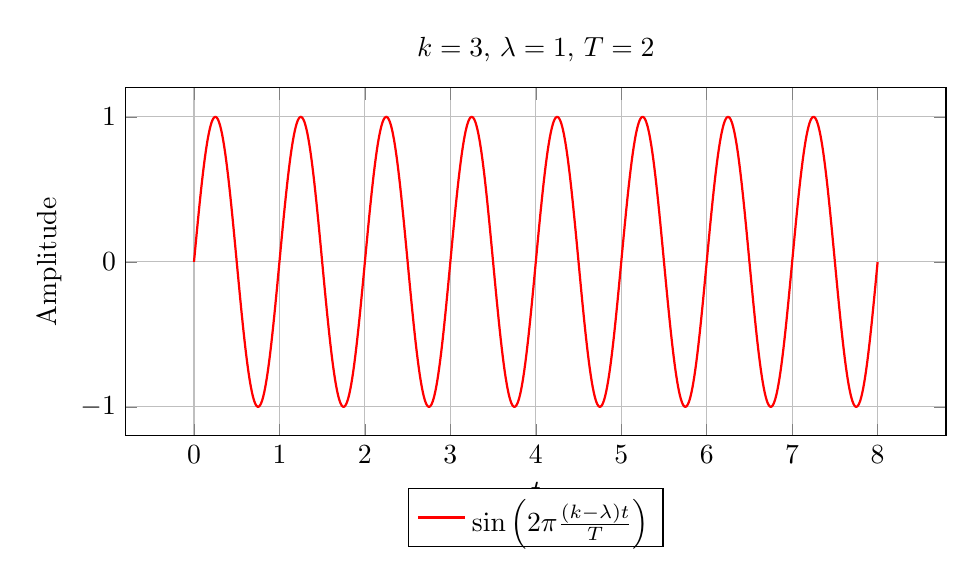
\begin{tikzpicture}
            \begin{axis}[
                width=12cm,
                height=6cm,
                grid=both,
                title={$k=3$, $\lambda=1$, $T=2$},
                xlabel={$t$},
                ylabel={Amplitude},
                legend style={at={(0.5,-0.15)}, anchor=north,legend columns=-1},
            ]
                \addplot[red, thick, domain=0:8, samples=1000] {sin(deg(2*pi*(3-1)*x/2))};
                \addlegendentry{$\sin\left(2\pi \frac{(k-\lambda)t}{T}\right)$}
            \end{axis}
        \end{tikzpicture}
        \end{center}
    \begin{itemize}
        \item \textbf{Note:} These plots show that for any length interval $T$, the integral (i.e. area under the curve) is 0. 
    \end{itemize}
\end{derivation}

\subsection{Analysis and Synthesis equation}
\begin{definition}
    \underline{Analysis equation}: Suppose $x(t) = \sum_{k \in \mathbb{Z}} c_k e^{j 2\pi \frac{k}{T} t}$.

    For any $\lambda \in \mathbb{Z}$,
    \[
    c_k = \frac{1}{T} \int_T x(t) e^{-j 2\pi \frac{k}{T} t} \, dt.
    \]
    \begin{itemize}
        \item \textbf{Intuition:} Given $x(t)$, analyze $x(t)$ and extract $c_k$ (i.e. FS coefficients) using the inner product and notion of orthgonality.
        \item \textbf{Note:} Don't forget that the basis set is conjugated.
    \end{itemize}
\end{definition}

\begin{derivation}
    Suppose $x(t) = \sum_{k \in \mathbb{Z}} c_k e^{j 2\pi \frac{k}{T} t}$.

    For any $\lambda \in \mathbb{Z}$,
    \begin{align*}
        \left\langle x(t), e^{j 2\pi \frac{\lambda}{T} t} \right\rangle &= \left\langle \sum_{k \in \mathbb{Z}} c_k e^{j 2\pi \frac{k}{T} t}, e^{j 2\pi \frac{\lambda}{T} t} \right\rangle \\
        &= \sum_{k \in \mathbb{Z}} c_k \left\langle e^{j 2\pi \frac{k}{T} t}, e^{j 2\pi \frac{\lambda}{T} t} \right\rangle \quad \text{Only when $k=\lambda$, the inner product is 1}\\
        &= c_\lambda \quad \text{by orthogonality, it picks out the $c_\lambda$ coefficient}
    \end{align*}

    Thus, to find the Fourier series coefficients,
    \[
    c_\lambda = \left\langle x(t), e^{j 2\pi \frac{\lambda}{T} t} \right\rangle \equiv c_k = \left\langle x(t), e^{j 2\pi \frac{k}{T} t} \right\rangle \quad \text{for any } k \in \mathbb{Z}.
    \]
\end{derivation}

\begin{definition}
    \underline{Synthesis equation}:
    \[
    x(t) \overset{a.e.}{=} \sum_{k \in \mathbb{Z}} c_k e^{j 2\pi \frac{k}{T} t}.
    \]
    \begin{itemize}
        \item \textbf{Intuition:} Given $c_k$, synthesize the signal using a linear combination of the basis set. 
    \end{itemize}
\end{definition}

\begin{warning}
    These are the go-to equations for solving Fourier series. 
    \begin{itemize}
        \item \textbf{Key:} $x(t)$ needs to be in this form (i.e. have a Fourier series representation) to use these equations. 
    \end{itemize}
\end{warning}

\begin{example}
    \customFigure[0.75]{00_Images/SQWAVE.png}{Square wave.}
    Take $x(t)$ as T-periodic where 
    \begin{align*}
        x(t) = 
        \begin{cases}
            0, & -\frac{T}{2} < t \leq -\frac{1}{2} \\
            \\
            1, & -\frac{1}{2} < t \leq \frac{1}{2} \\
            \\
            0, & \frac{1}{2} < t \leq \frac{T}{2}
        \end{cases}
        , \quad \text{extend periodically}.
    \end{align*}
    
    \begin{align*}
        x(t) &= \sum_{k=-\infty}^{\infty} c_k e^{j2\pi \frac{k}{T} t}, \quad \text{with } c_k = \frac{1}{T} \int_{T} x(t) e^{-j2\pi \frac{k}{T} t} \, dt
    \end{align*}

    For $k=0$:
    \begin{align*}
        c_0 &= \int_{-1/2}^{1/2} 1 dt \\ 
        &= \frac{1}{T} \left(\frac{1}{2} + \frac{1}{2}\right) \\
        &= \frac{1}{T}
    \end{align*}
    
    For $k\neq 0$
    \begin{align*}
        c_k &= \frac{1}{T} \int_{-\frac{1}{2}}^{\frac{1}{2}} e^{-j2\pi \frac{k}{T} t} \, dt \\
        &= \frac{1}{T} \left( \frac{1}{-j2\pi k/T} e^{-j2\pi \frac{k}{T} t} \Big|_{-\frac{1}{2}}^{\frac{1}{2}} \right) \\
        &= \frac{1}{T} \left( \frac{T}{-j2\pi k} \left( e^{-j2\pi \frac{k}{T} \left(\frac{1}{2}\right)} - e^{-j2\pi \frac{k}{T} \left(-\frac{1}{2}\right)} \right) \right) \\
        &= \frac{1}{T} \cdot \frac{T}{j 2\pi k} \left(e^{j \pi \frac{k}{T}} - e^{-j \pi \frac{k}{T}} \right) \quad \text{putting negative into brackets}\\
        &= \frac{1}{T} \cdot \frac{1}{\pi k / T} \sin \left(\frac{\pi k}{T}\right) \quad \text{where } \sin\theta = \frac{1}{2j} \left(e^{j\theta} - e^{-j\theta}\right)\\
        c_k &= \frac{1}{T} \text{sinc}\left(\frac{\pi k}{T}\right), \quad \text{(sinc function definition $\text{sinc} (x) \overset{\Delta}{=} \frac{\sin (\pi x)}{\pi x}$)}
    \end{align*}
    \vspace{1em}
    
    \textbf{Sinc Function Plot}

    \begin{align*}
        \text{sinc}(x) &\triangleq \frac{\sin(\pi x)}{\pi x} \\
        &= \frac{1}{\pi x} \left( \pi x - \frac{(\pi x)^3}{3!} + \frac{(\pi x)^5}{5!} - \ldots \right) \\
        &= 1 - \frac{(\pi x)^2}{3!} + \frac{(\pi x)^4}{5!} - \ldots
    \end{align*}
    
    \begin{center}
    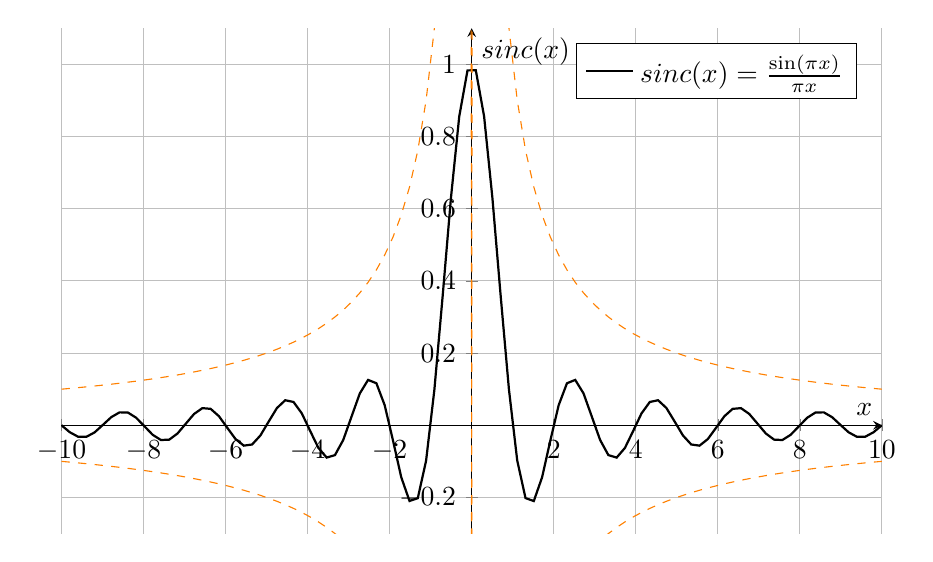
\begin{tikzpicture}
        \begin{axis}[
            axis lines=middle,
            xlabel={$x$},
            ylabel={$\text{sinc}(x)$},
            samples=100,
            domain=-10:10,
            xmin=-10, xmax=10,
            ymin=-0.3, ymax=1.1,
            width=12cm, height=8cm,
            grid=both,
            legend pos=north east
        ]
        \addplot[thick, black] {sin(deg(pi*x))/(pi*x)};
        \addlegendentry{$\text{sinc}(x) = \frac{\sin(\pi x)}{\pi x}$}
        \addplot[dashed, orange] {1/x};
        \addplot[dashed, orange] {-1/x};
        \end{axis}
    \end{tikzpicture}
    \end{center}
    \begin{itemize}
        \item \textbf{Note:} Goes through 0 at integer values except for at $x=0$.
    \end{itemize}
    \vspace{1em}

    \textbf{Visualization of FS Coefficients}
    \customFigure[0.5]{00_Images/FSC.png}{Fourier series coefficients at $T=4$}
    
    \vspace{1em}

    
    \textbf{Final form:}
    \begin{align*}
        x(t) &= c_0 + 2 c_1 \left( \frac{e^{j2\pi \frac{1}{T} t} + e^{-j2\pi \frac{1}{T} t}}{2} \right) + 2 c_2 \left( \frac{e^{j2\pi \frac{2}{T} t} + e^{-j2\pi \frac{2}{T} t}}{2} \right) + \ldots \\
        x(t) &= c_0 + \sum_{k=1}^{\infty} \frac{2}{T} \text{sinc} \left( \frac{k}{T} \right) \cos \left( 2\pi \frac{k}{T} t \right)
    \end{align*}
    
    \begin{itemize}
        \item Added \(\frac{2}{2}\) to introduce \(\cos\theta = \frac{1}{2} \left(e^{j \theta} - e^{-j \theta}\right) \)
        \item $c_{-k} = c_k = \frac{1}{T} \text{sinc} \left( \frac{k}{T} \right)$
        \item \(2c_k\): $\frac{2}{T} \text{sinc} \left( \frac{k}{T} \right)$
        \item Basis set: $\cos \left( 2\pi \frac{k}{T} t \right)$
    \end{itemize}
    \vspace{1em}
    
    \textbf{Consider a Truncated Series:}
    \begin{align*}
        x_N(t) = \frac{1}{T} + \sum_{k=1}^{N} \frac{2}{T} \text{sinc} \left( \frac{k}{T} \right) \cos \left( 2\pi \frac{k}{T} t \right)
    \end{align*}
    
    \customFigure[0.75]{00_Images/GP.png}{Gibb's Phenomenon}

    \customFigure[0.75]{00_Images/NUC.png}{Non-uniform convergence}
    \begin{itemize}
        \item \textbf{Gibb's Phenomenon:} There is a 9\% overshoot on either end of the jump discontinuity. The overshoot does not disappear as more terms are added, but the width of the overshoot region becomes smaller.
        \item \textbf{Non-uniform convergence:} When a series converges to a function at different rates across its domain, meaning that convergence is slower in certain regions (i.e. overshoots) and faster on the flat regions. 
    \end{itemize}
\end{example}